\documentclass[10pt]{article}
\usepackage{tocloft}
\usepackage{adjustbox}
\usepackage{blindtext}
\usepackage{titlesec}
\usepackage[margin=1in]{geometry}
\usepackage{amsmath}
\usepackage{amsthm}
\usepackage{amssymb}
\usepackage{float}
\usepackage{graphics}
\usepackage{graphicx}
\usepackage{caption}
\usepackage[normalem]{ulem}
\usepackage{enumitem}
\usepackage{natbib}
\usepackage{sectsty}
\usepackage{subcaption}
\usepackage{csvsimple}
\usepackage{tikz}
\usetikzlibrary{shapes.geometric}
\usetikzlibrary{trees}
\usepackage{hyperref}
\hypersetup{
        colorlinks = true,
        linkcolor = blue,
        filecolor = magenta,            
        urlcolor = cyan,
        pdftitle={Overleaf Example},
        pdfpagemode=FullScreen,
}

\title{Homework 2: Classification \& Language Modeling}
\author{Isaac Thomas}
\setcounter{tocdepth}{5}
\setcounter{secnumdepth}{5}
\setcounter{section}{0}

\newcommand{\code}[1]{\texttt{#1}}

\makeatletter
\renewcommand\paragraph{\@startsection{subparagraph}{5}{\parindent}%
        {3.25ex \@plus1ex \@minus .2ex}%
        {0.75ex plus 0.1ex}% space after heading
        {\normalfont\normalsize\bfseries}}
\makeatother

\makeatletter

\newcommand{\dateformatter}[2]{%
    \textbf{#1} -- \textit{#2}%
}

\newcommand{\dateevent}[2]{%
    \addcontentsline{dates}{section}{#1 -- #2}%
    \dateformatter{#1}{#2}%
}

\newcommand{\listofdates}{%
    \begingroup
    \renewcommand{\contentsname}{List of Dates}
    \let\old@starttoc\@starttoc
    \def\@starttoc##1{%
        \old@starttoc{dates}%
    }
    \tableofcontents%
    \endgroup
}

\makeatother

%\AddToHook{cmd/section/before}{\clearpage}
\sectionfont{\fontsize{12}{15}\selectfont}
\subsectionfont{\fontsize{10}{15}\selectfont}

\theoremstyle{definition}
\newtheorem{definition}{Definition}
\newtheorem{lemma}{Lemma}
\DeclareSymbolFont{matha}{OML}{txmi}{m}{it}% txfonts
\DeclareMathSymbol{\varv}{\mathord}{matha}{118}
\newcommand{\Setup}{\code{Setup}}
\newcommand{\Prove}{\code{Prove}}
\newcommand{\Verify}{\code{Verify}}
\newcommand{\Sim}{\code{Sim}}
\setlistdepth{100}
\newenvironment{myenum}%
{\pointedenum\begin{enumerate}}%
{\end{enumerate}}
\begin{document}
\maketitle

\section{Problem 1: Speech Classification}
\noindent For this classification problem - namely, predict which president said a given sentence - we used a transformer encoder classifier consisting of:
\begin{itemize}
    \item a composite embedding which uses \code{torch.nn.Embedding} and a sinusoidal positional encoding to map each token to a high-dimension latent representation
    \item multiple sequential \textbf{encoder} blocks, each of which uses multi-head attention to extract contextual relationships between tokens
    \item a fully connected layer producing a one-hot vector corresponding to the predicted class
\end{itemize}

\noindent The training and evaluation dataset consisted of numerous sentences, each of which was uttered by one of three presidents. We trained this model (\code{epochs=15}, \code{batch\_size}=16) on the former dataset using an adam optimizer with a learning rate of $\alpha = 0.001$. The resulting model achieved an accuracy of $86.8\%$ on the evaluation dataset. Below is a table depicting the progression of training loss/accuracy:\\
\begin{center}
\csvautotabular{../data/training_metrics/transformer_encoder.csv}
\end{center}

\noindent We accompany this data with visualized attention maps from the last of each encoder's attention heads. The corresponding plots below depict which tokens were found to have strong contextual relationships:

\begin{figure}[H]
    \centering
    \begin{subfigure}[b]{0.35\textwidth}
        \centering
        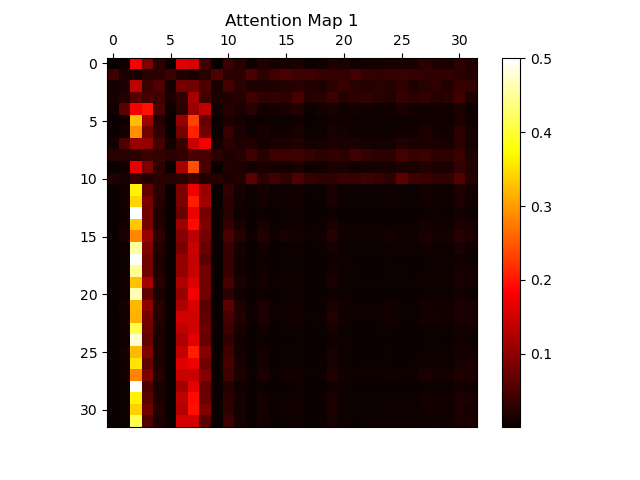
\includegraphics[scale=0.4]{../data/plots/part1/attention_map_1.png}
        \label{subfig:am1}
    \end{subfigure}
    \begin{subfigure}[b]{0.35\textwidth}
        \centering
        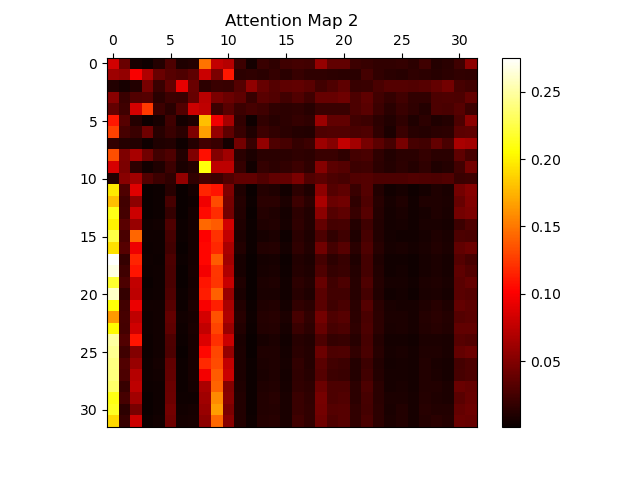
\includegraphics[scale=0.4]{../data/plots/part1/attention_map_2.png}
        \label{subfig:am2}
    \end{subfigure}
    \begin{subfigure}[b]{0.35\textwidth}
        \centering
        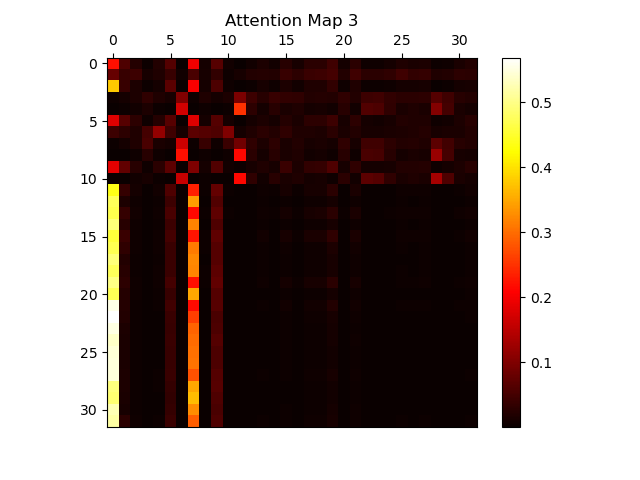
\includegraphics[scale=0.4]{../data/plots/part1/attention_map_3.png}
        \label{subfig:am3}
    \end{subfigure}
    \begin{subfigure}[b]{0.35\textwidth}
        \centering
        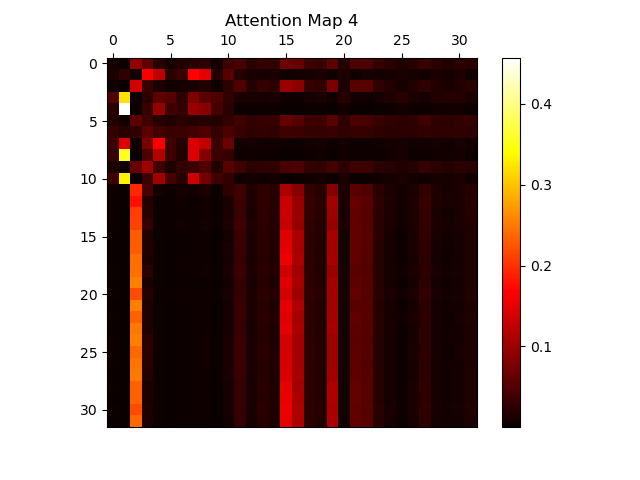
\includegraphics[scale=0.4]{../data/plots/part1/attention_map_4.png}
        \label{subfig:am4}
    \end{subfigure}
\caption{the \code{n\_head}-th attention map from each encoder layer in the transformer encoder. The progressive acquisition of contextual relationships between the tokens in the training data is visible from the increase in cell intensity from layer to layer.}
\end{figure}
\noindent Along with the generally increasing understanding of token-wise relationships, we see that tokens have affinity towards preceding tokens; this is visible from the intensities being much stronger in the first few columns than in the first few rows. This aligns with our natural understanding of the english language, as the contextual meaning of a word is derived from preceding words in the same sentence. That being said, some acquisition of context from future tokens is also visible. We should expect not to see such a thing in the decoder model we implement due to the masking in the self-attention heads. Additionally, it seems there is abundant affinity between too many pairs of tokens. Applying dropout while maintaining the total "attention mass" one token can "pay" to other tokens could force the network to focus more on the token relationships that matter at the expense of the rest. We will discuss this more in part 3.


\section{Problem 2: Language Modeling}
This language modeling problem involves predicting the most likely following token based on information from previous tokens. For this task we used a transformer decoder consisting of:
\begin{itemize}
    \item a composite embedding which uses \code{torch.nn.Embedding} and a sinusoidal absolute positional encoding to map each token to a high-dimension latent representation.
    \item multiple sequential \textbf{decoder} blocks, each of which uses masked multi-head self- attention to extract contextual relationships between a given token and those preceding it
    \item a fully connected layer, which produces a one-hot vector indicating the most likely token in our vocabulary to come next \textbf{for each token in the given sequence}
\end{itemize}

\noindent The training dataset consisted of numerous sentences, each of which was tokenized and collated into batches before training like in the first problem. The test datasets were speech corpi from George H. Bush, Barack Obama, and George W. Bush respectively. We trained this model (\code{epochs=15}, \code{batch\_size}=16) on the first of these four datasets using an adam optimizer with a learning rate of $\alpha = 0.001$. We depict the training loss/perplexity every 100 iterations below, as well as the final test perplexities on the three test datasets.
% \begin{figure}[H]
% \begin{center}
% \csvautotabular{../data/training_metrics/transformer_decoder.csv}
% \end{center}

\noindent We accompany this data with visualized attention maps from the last of each encoder's attention heads. The corresponding plots below depict which tokens were found to have strong contextual relationships:

\begin{figure}[H]
    \centering
    \begin{subfigure}[b]{0.35\textwidth}
        \centering
        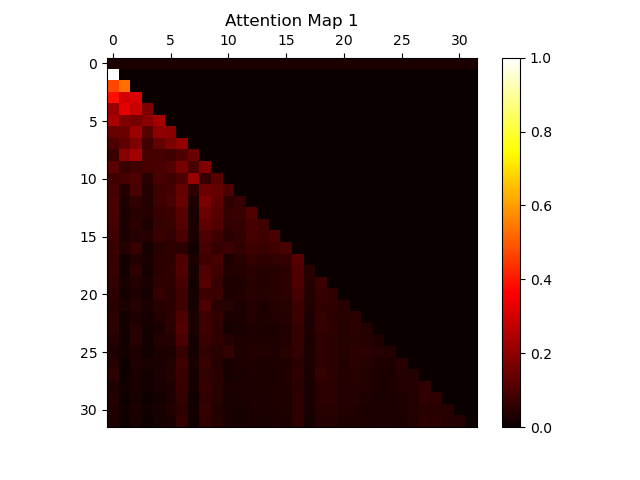
\includegraphics[width=\textwidth]{../data/plots/part2/attention_map_1.png}
        \label{subfig:am1}
    \end{subfigure}
    \begin{subfigure}[b]{0.35\textwidth}
        \centering
        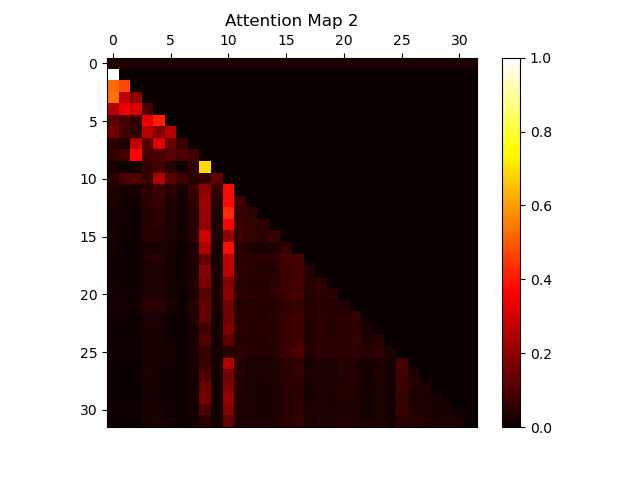
\includegraphics[width=\textwidth]{../data/plots/part2/attention_map_2.png}
        \label{subfig:am2}
    \end{subfigure}
    \begin{subfigure}[b]{0.35\textwidth}
        \centering
        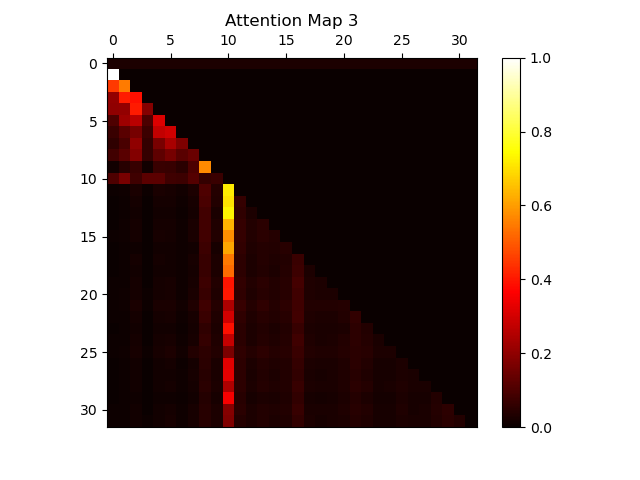
\includegraphics[width=\textwidth]{../data/plots/part2/attention_map_3.png}
        \label{subfig:am3}
    \end{subfigure}
    \begin{subfigure}[b]{0.35\textwidth}
        \centering
        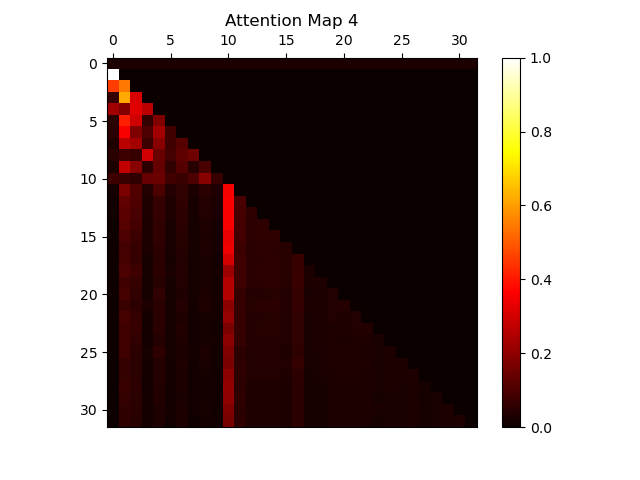
\includegraphics[width=\textwidth]{../data/plots/part2/attention_map_4.png}
        \label{subfig:am4}
    \end{subfigure}
\caption{the \code{n\_head}-th attention map from each encoder layer in the trained transformer decoder. As mentioned before, we only see nonzero affinities between the $i$-th token and the $j$-th token in a given block if $i > j$ (token $j$ precedes token $i$).}
\end{figure}
\section{Problem 3: Exploration}

\noindent We mentioned in part 1 that we could potentially improve the performance of the classifier by sharpening the focus of each decoder layer's attention heads. Exploring this option further, we applied dropout to the attention weights after applying the softmax function, then re-normalized the weights so they still summed up to 1 across each row (see \code{transformer.AttentionHead}). We then trained the resulting model on the same training dataset as in part 1 and computed the same training/evaluation metrics.

\bibliographystyle{plain}
\bibliography{references}
\end{document}